\documentclass[11pt]{exam}
\usepackage[margin=1in]{geometry}
\pagestyle{plain}
\usepackage{amsmath,amsfonts,amssymb,amsthm,enumerate}
\usepackage{multicol}
\usepackage[]{graphicx}
\usepackage{hyperref}
\usepackage{tikz}
\usepackage{pgfplots}
\usepackage{subfigure}
\usepackage[final]{pdfpages}

\addtolength{\footskip}{2\baselineskip} % to lower the page numbers
\title{\vspace{-0.5in} Math 115 \\ Worksheet Section
  4.5 continued}
\date{}


% \theoremstyle{definition}
% \newtheorem{problem}{Problem}
\renewcommand{\questionlabel}{\textbf{Problem~\thequestion.}}
\printanswers

\begin{document}
\maketitle
\section*{The basics}
\begin{itemize}
\item The {\bf cost function} $C(q)$ gives the cost of producing a
  quantity $q$ of a certain good.

 \item The {\bf revenue function} $R(q)$ gives the revenue received from
  selling a quantity $q$ of some good.

  \item The {\bf profit} $\pi(q)=R(q)-C(q)$ gives the total profit from
  producing and selling $q$ of that good.

  \item To decide whether a company's profit would increase or decrease if
  the company increased or decreased production of a certain good, we
  might look at the marginal cost and marginal revenue:

  \item The {\bf marginal cost} is given by
  $\textrm{MC}(q)= C'(q)\approx C(q+1)-C(q)$

  \item The {\bf marginal revenue} is given by
  $\textrm{MR}(q)= R'(q) \approx R(q+1)-R(q)$
\end{itemize}
\vspace{1em}

\noindent
When can maximum profit occur? \\

 Where marginal cost = marginal revenue, other critical points where
  MR or MC do not exist, and at endpoints \\

\noindent
How do we identify the fixed cost of producing a certain good? \\

The value of \(C(0)\).

\pagebreak
    \ifprintanswers 
    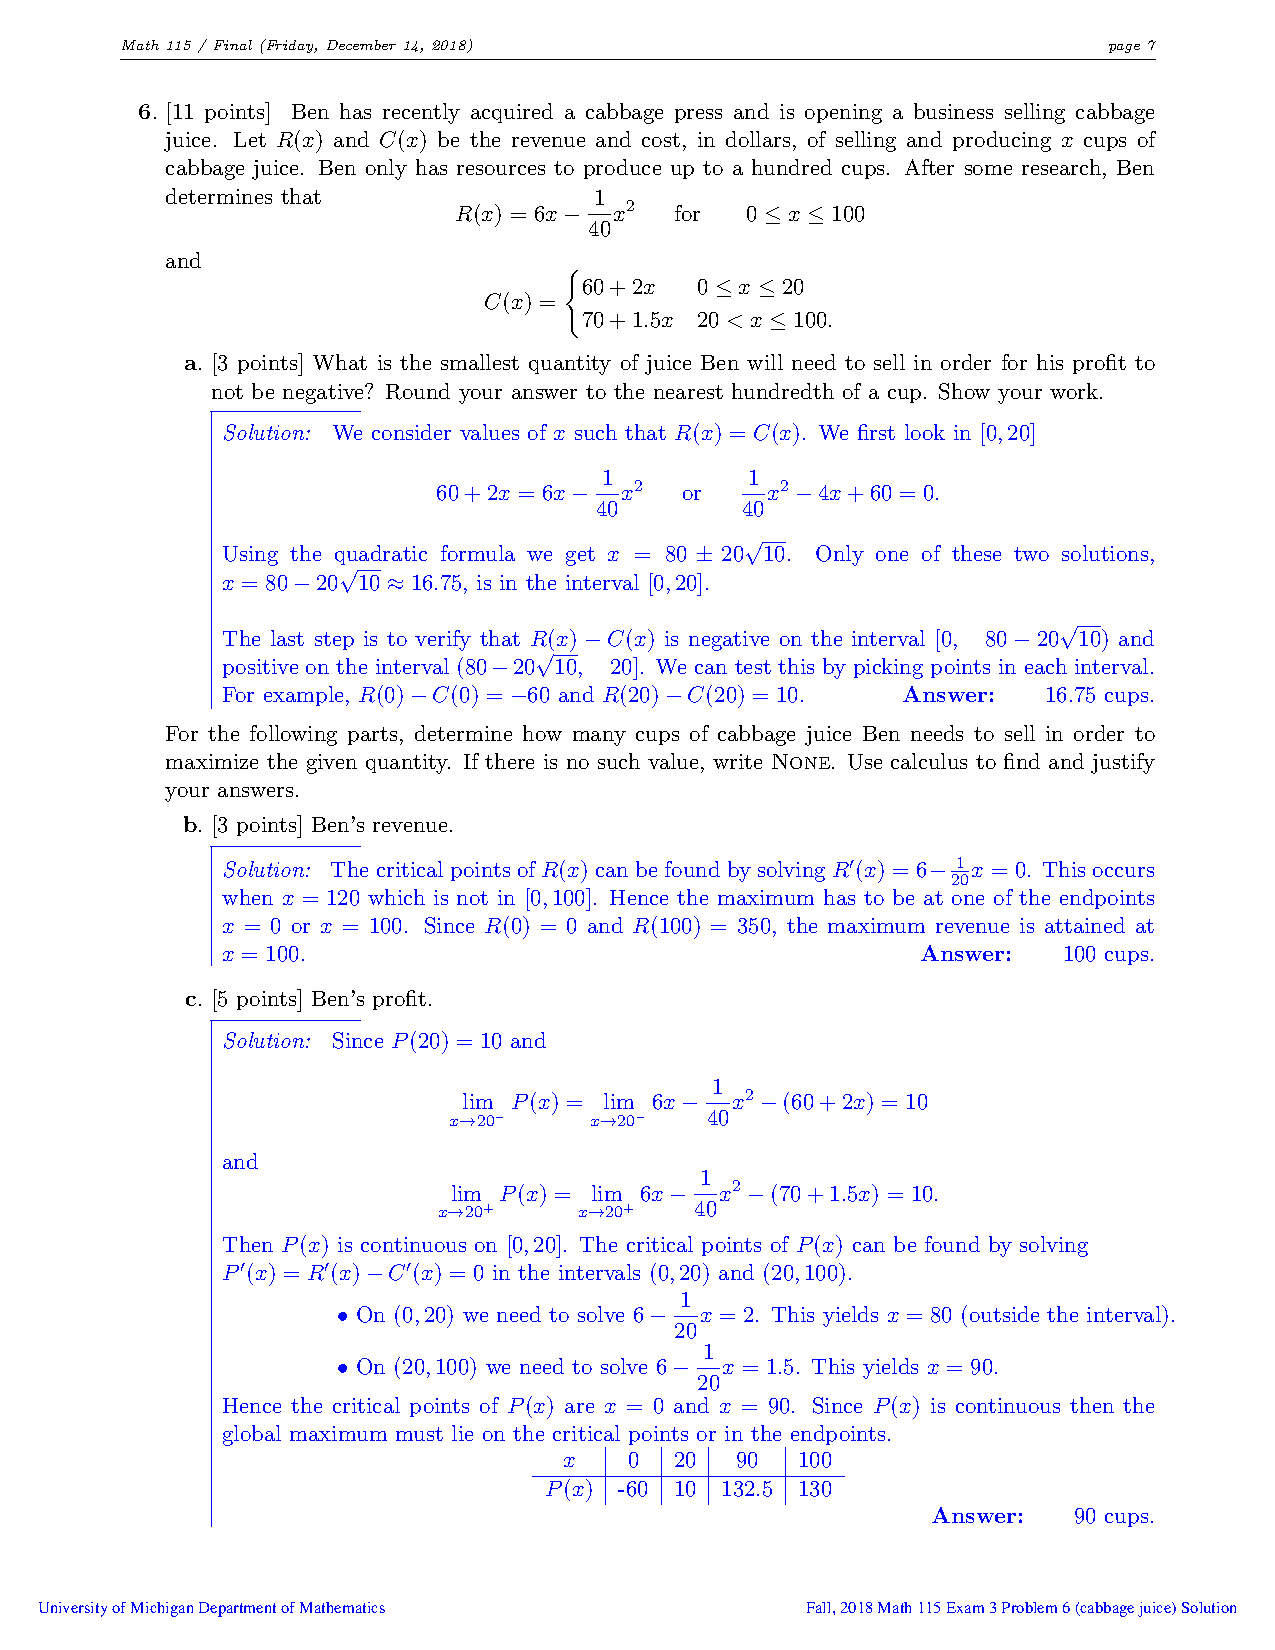
\includepdf[pages=-,pagecommand={}]{Figures/s6.pdf}
    \else
    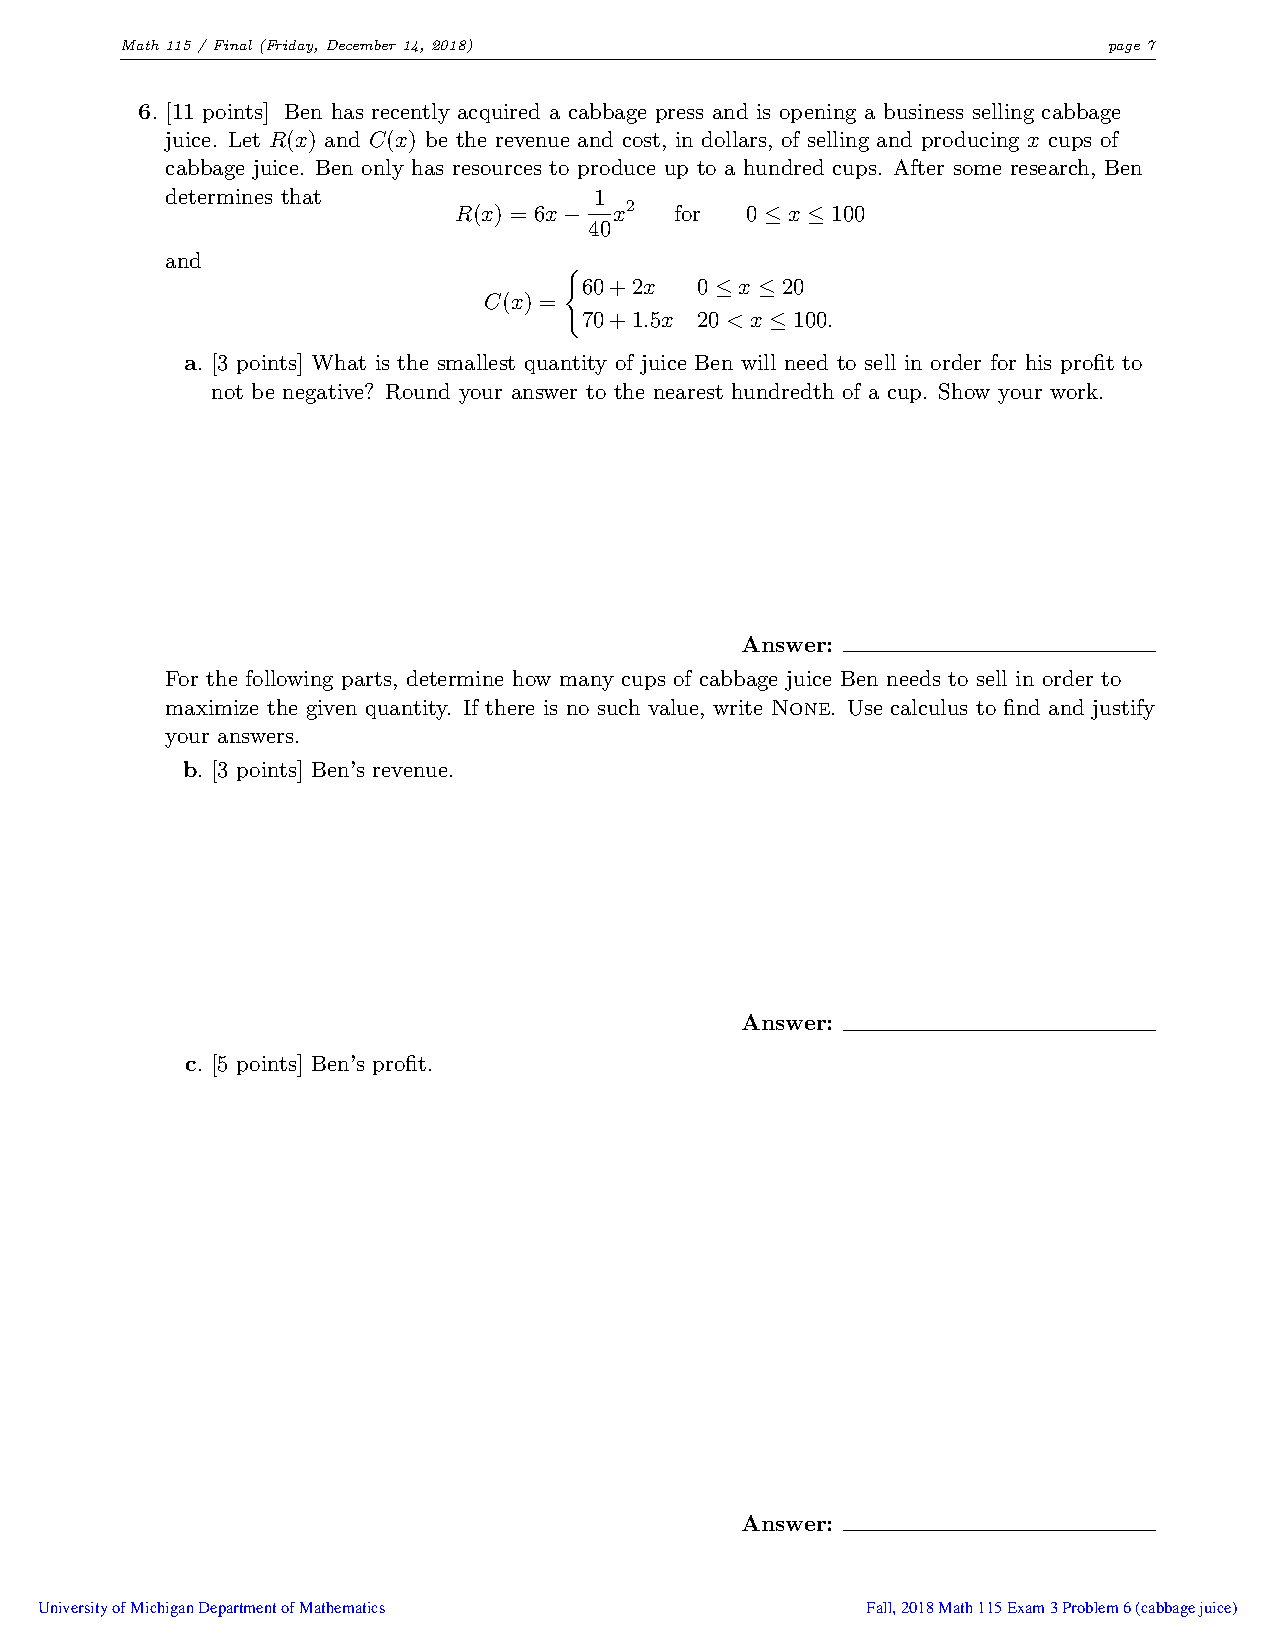
\includepdf[pages=-,pagecommand={}]{Figures/p6.pdf}
    \fi
\pagebreak
    \ifprintanswers 
    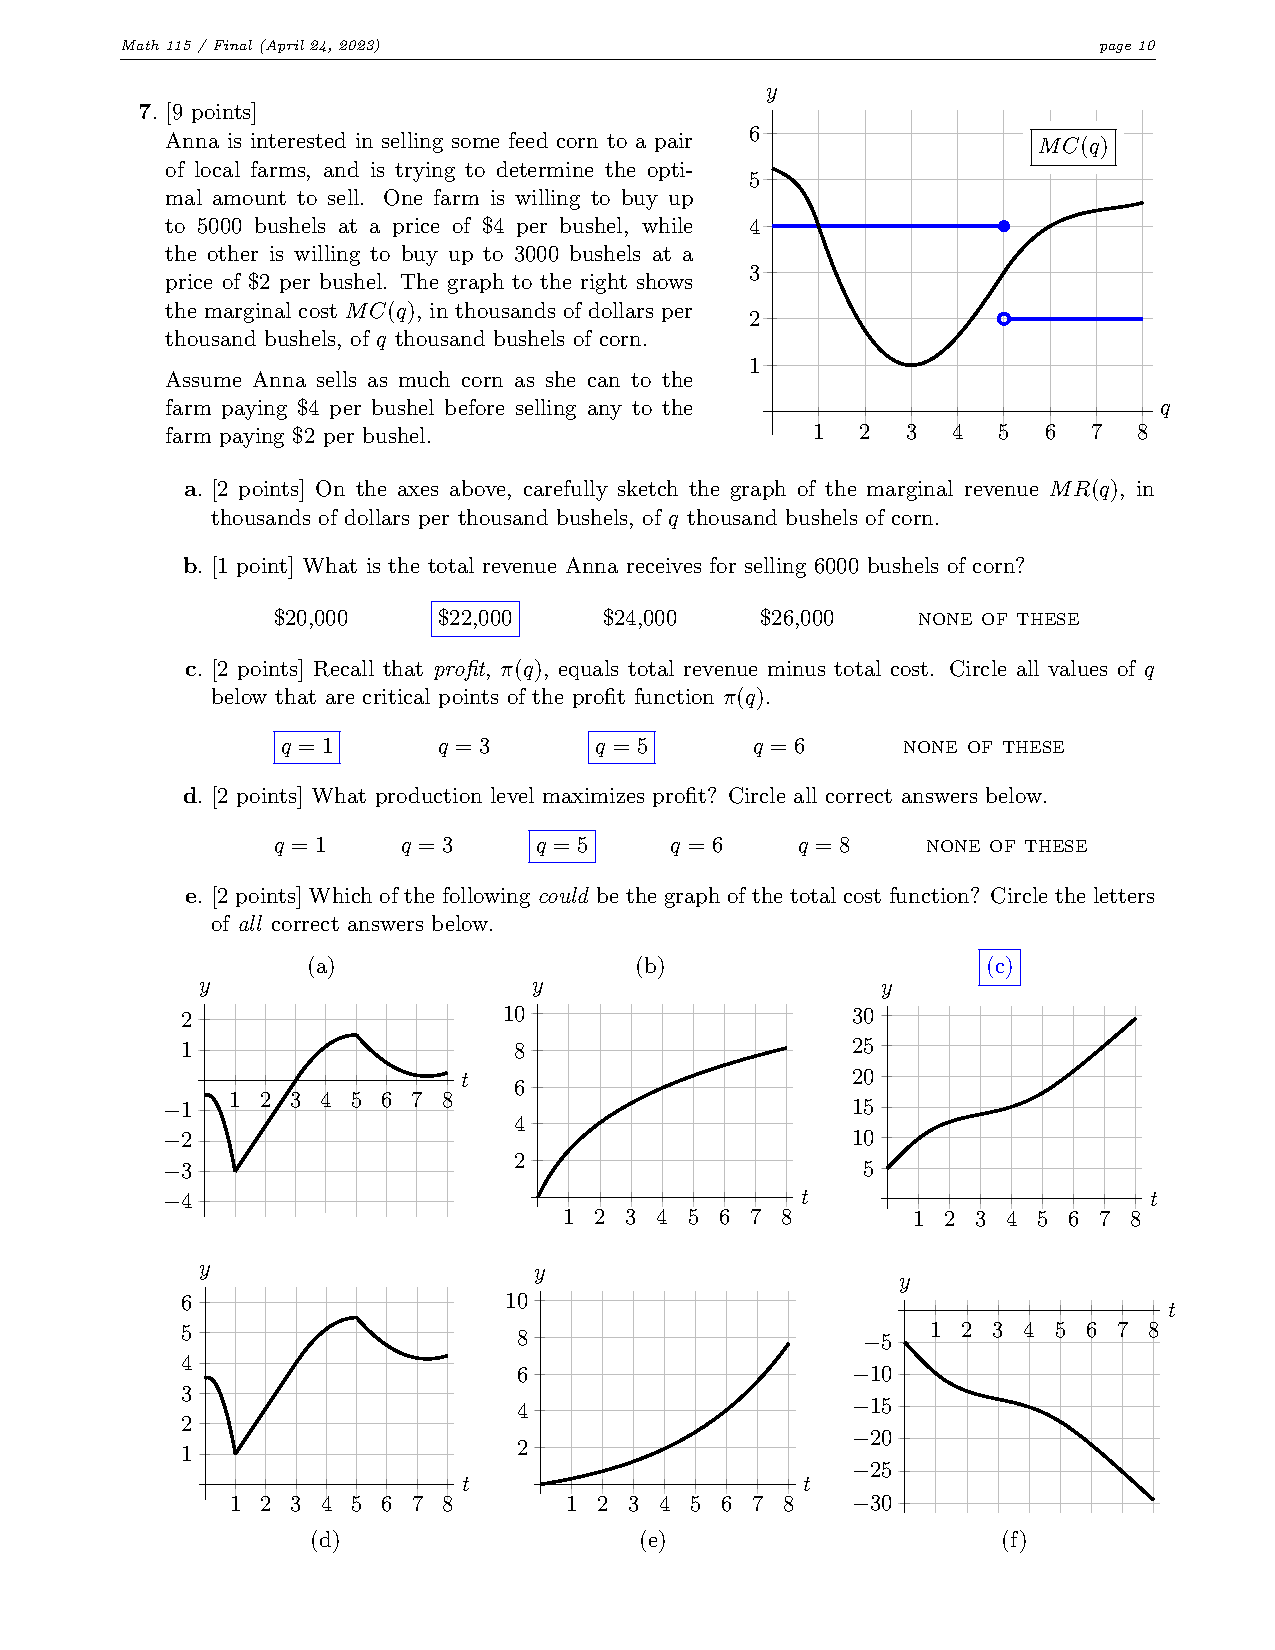
\includepdf[pages=-,pagecommand={}]{Figures/s7.pdf}
    \else
    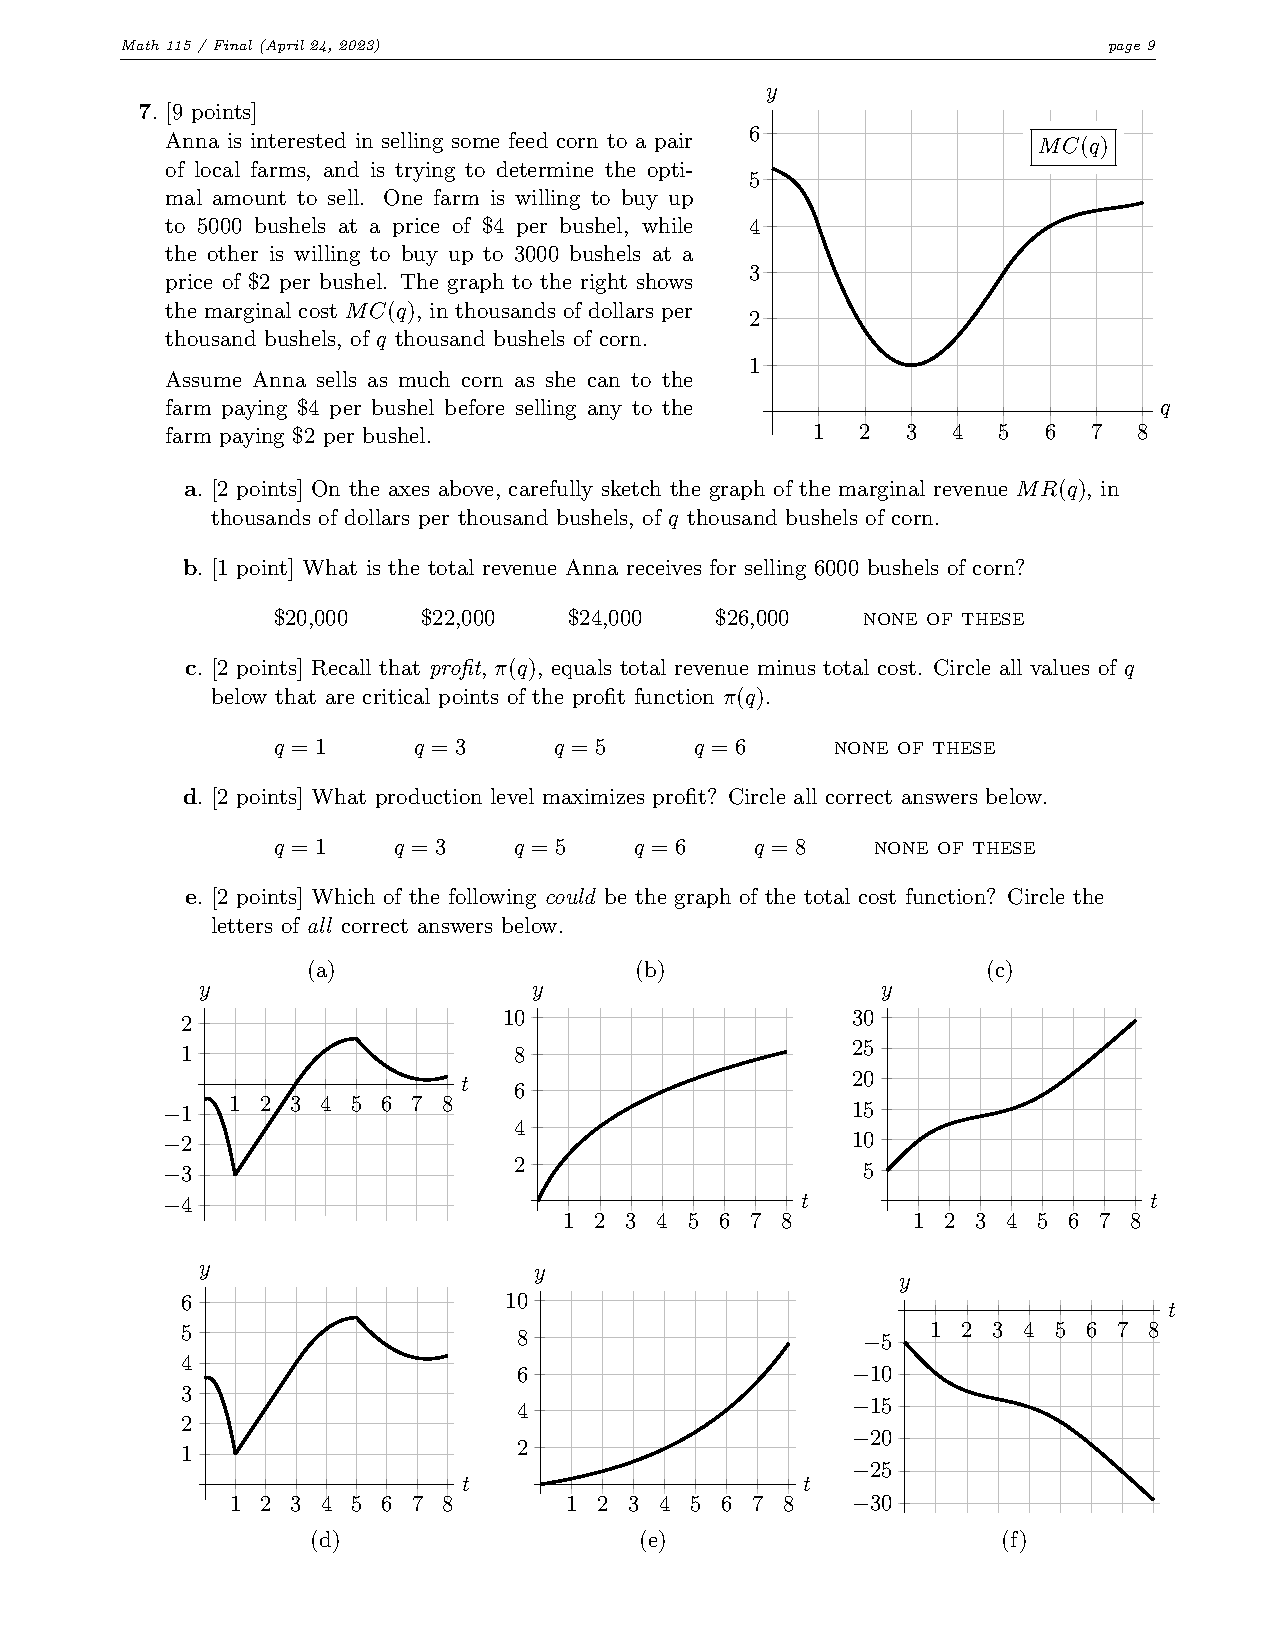
\includepdf[pages=-,pagecommand={}]{Figures/p7.pdf}
    \fi
\pagebreak
    \ifprintanswers 
    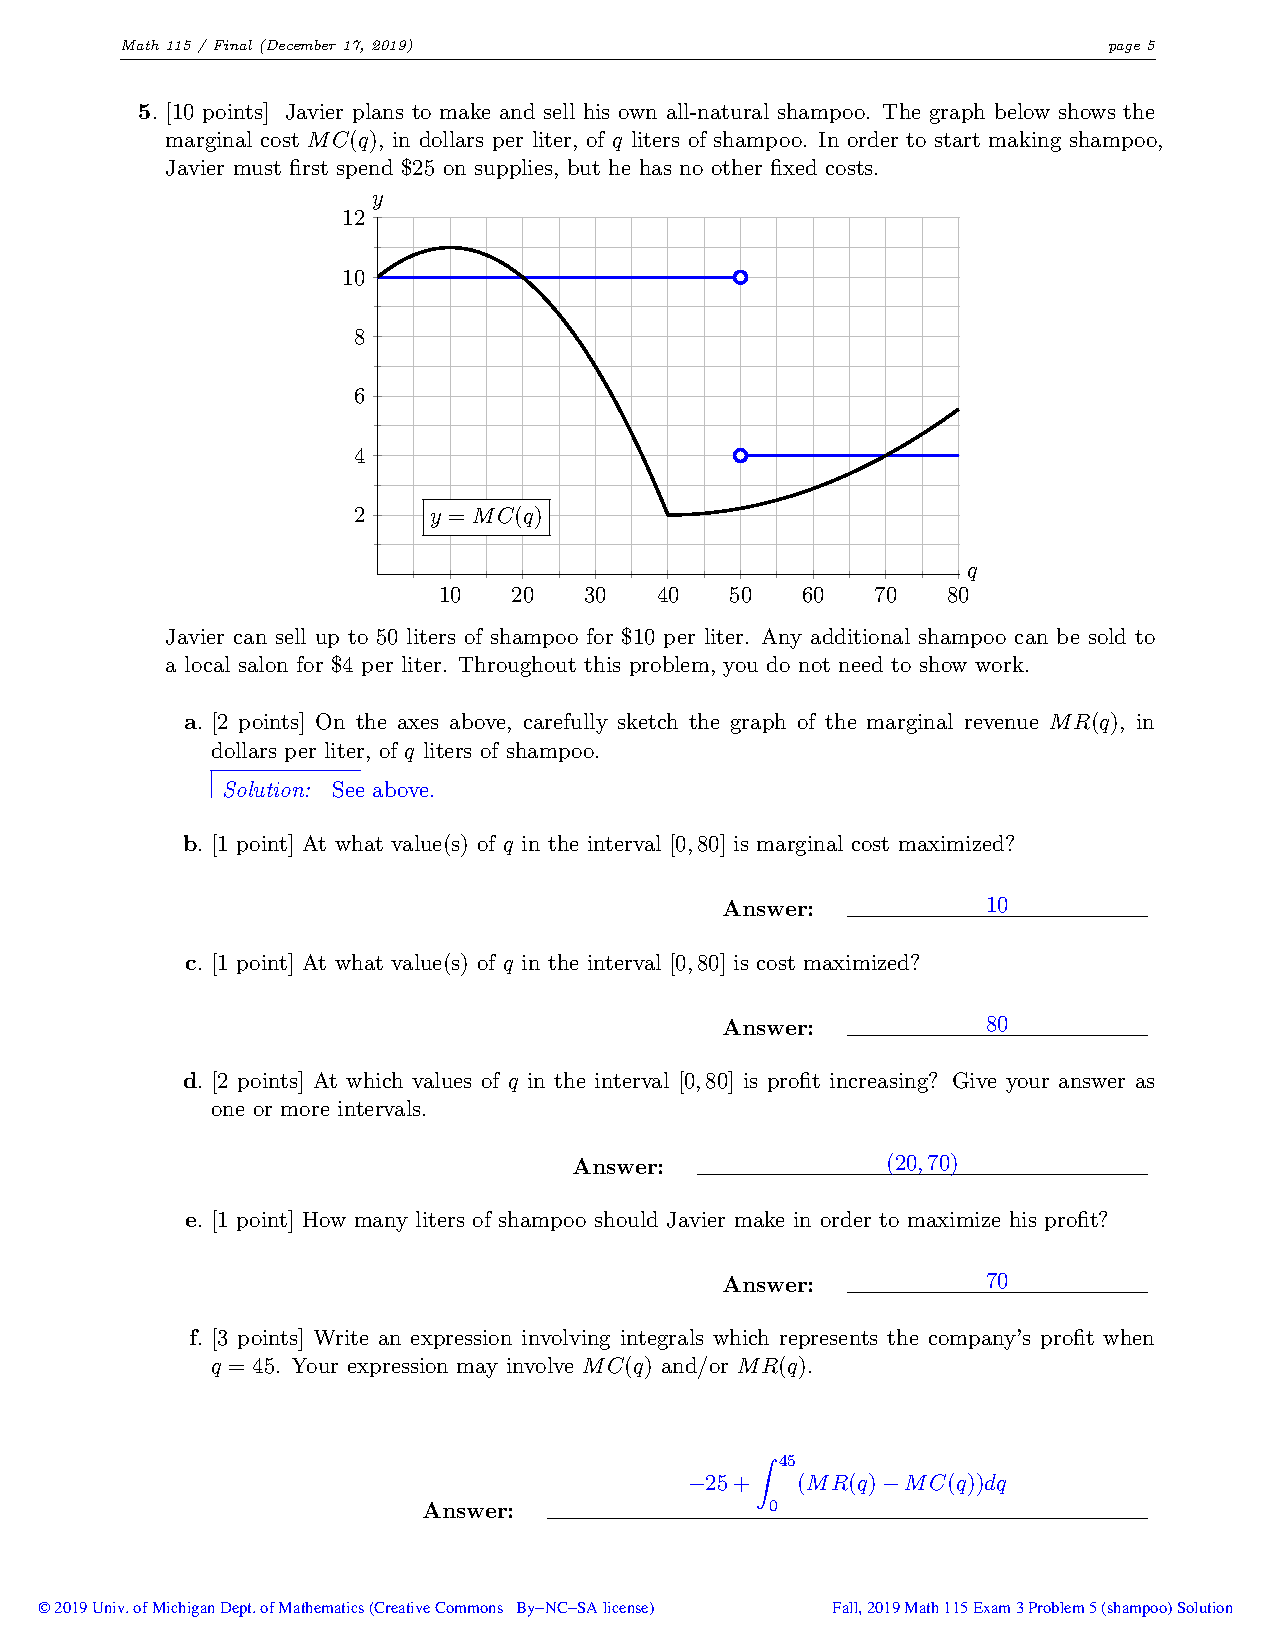
\includepdf[pages=-,pagecommand={}]{Figures/s5.pdf}
    \else
    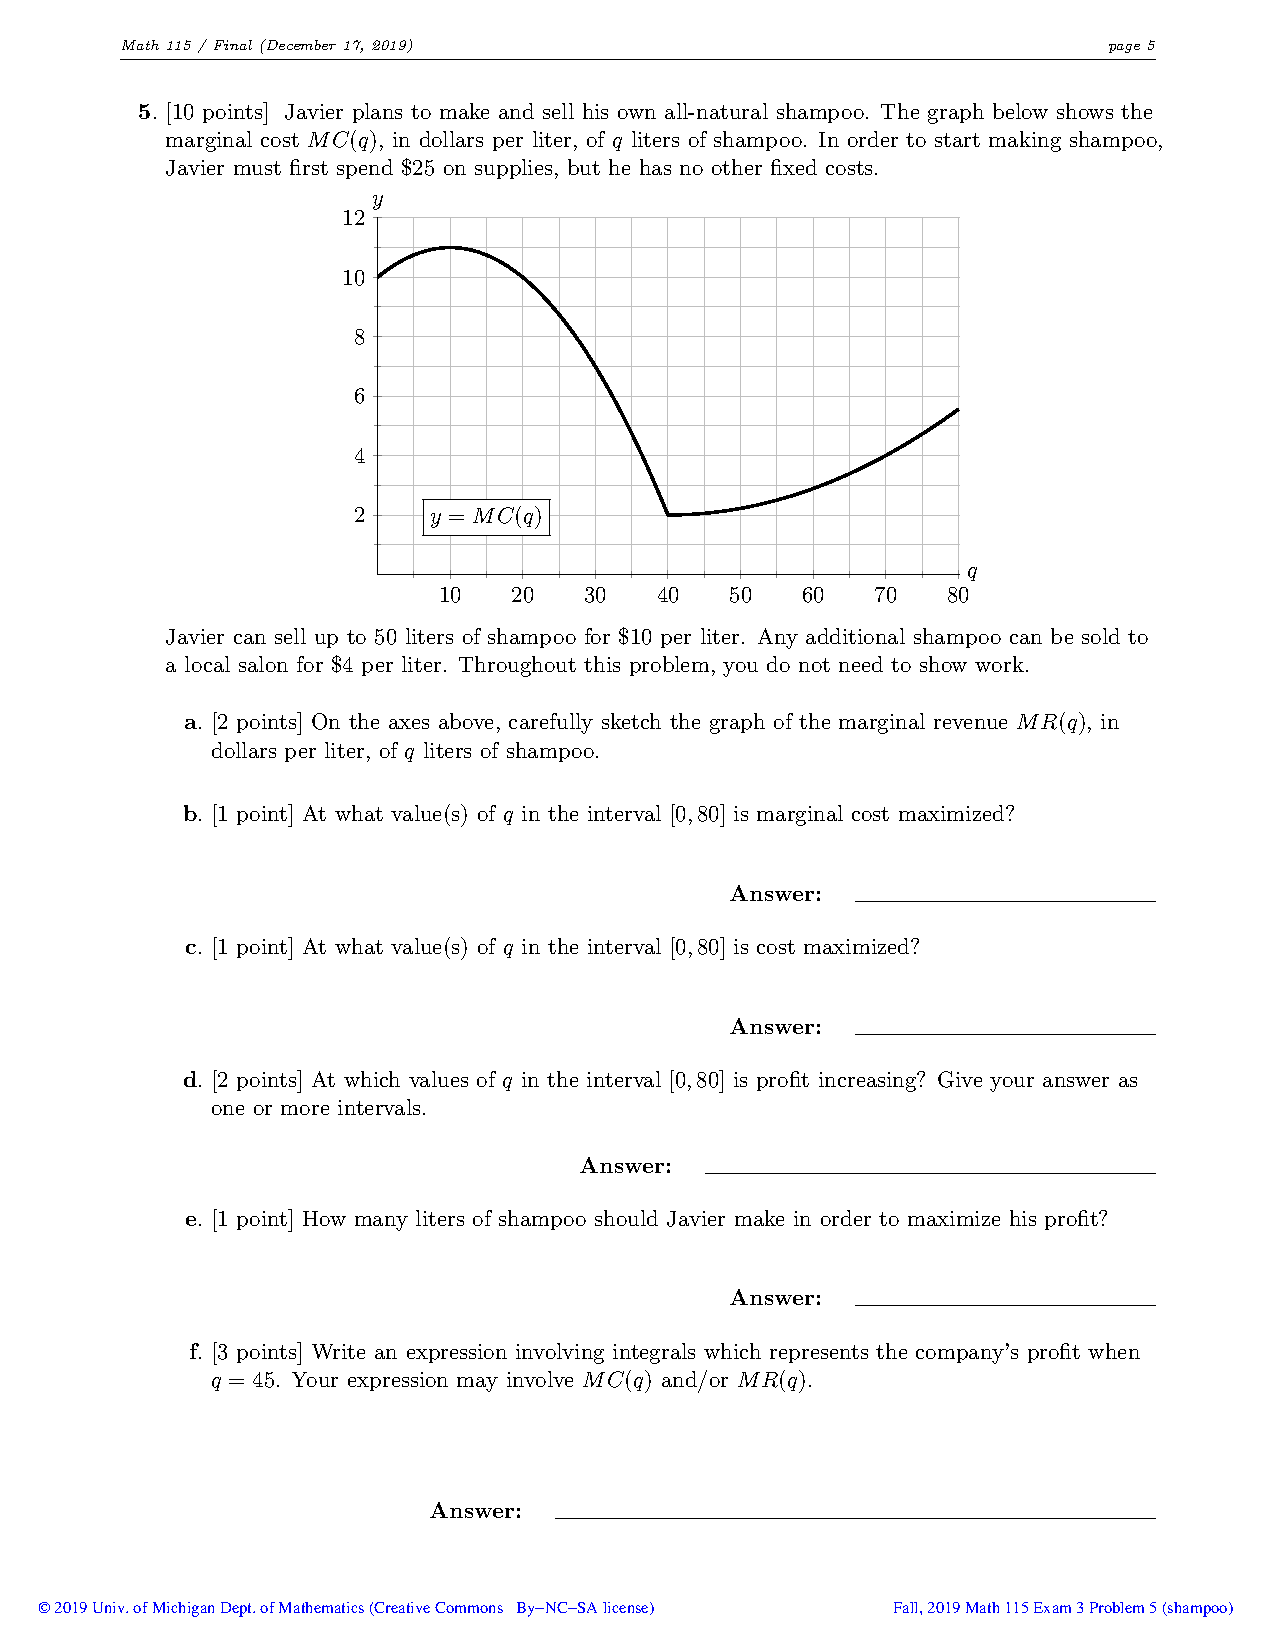
\includepdf[pages=-,pagecommand={}]{Figures/p5.pdf}
    \fi
\pagebreak
    \ifprintanswers 
    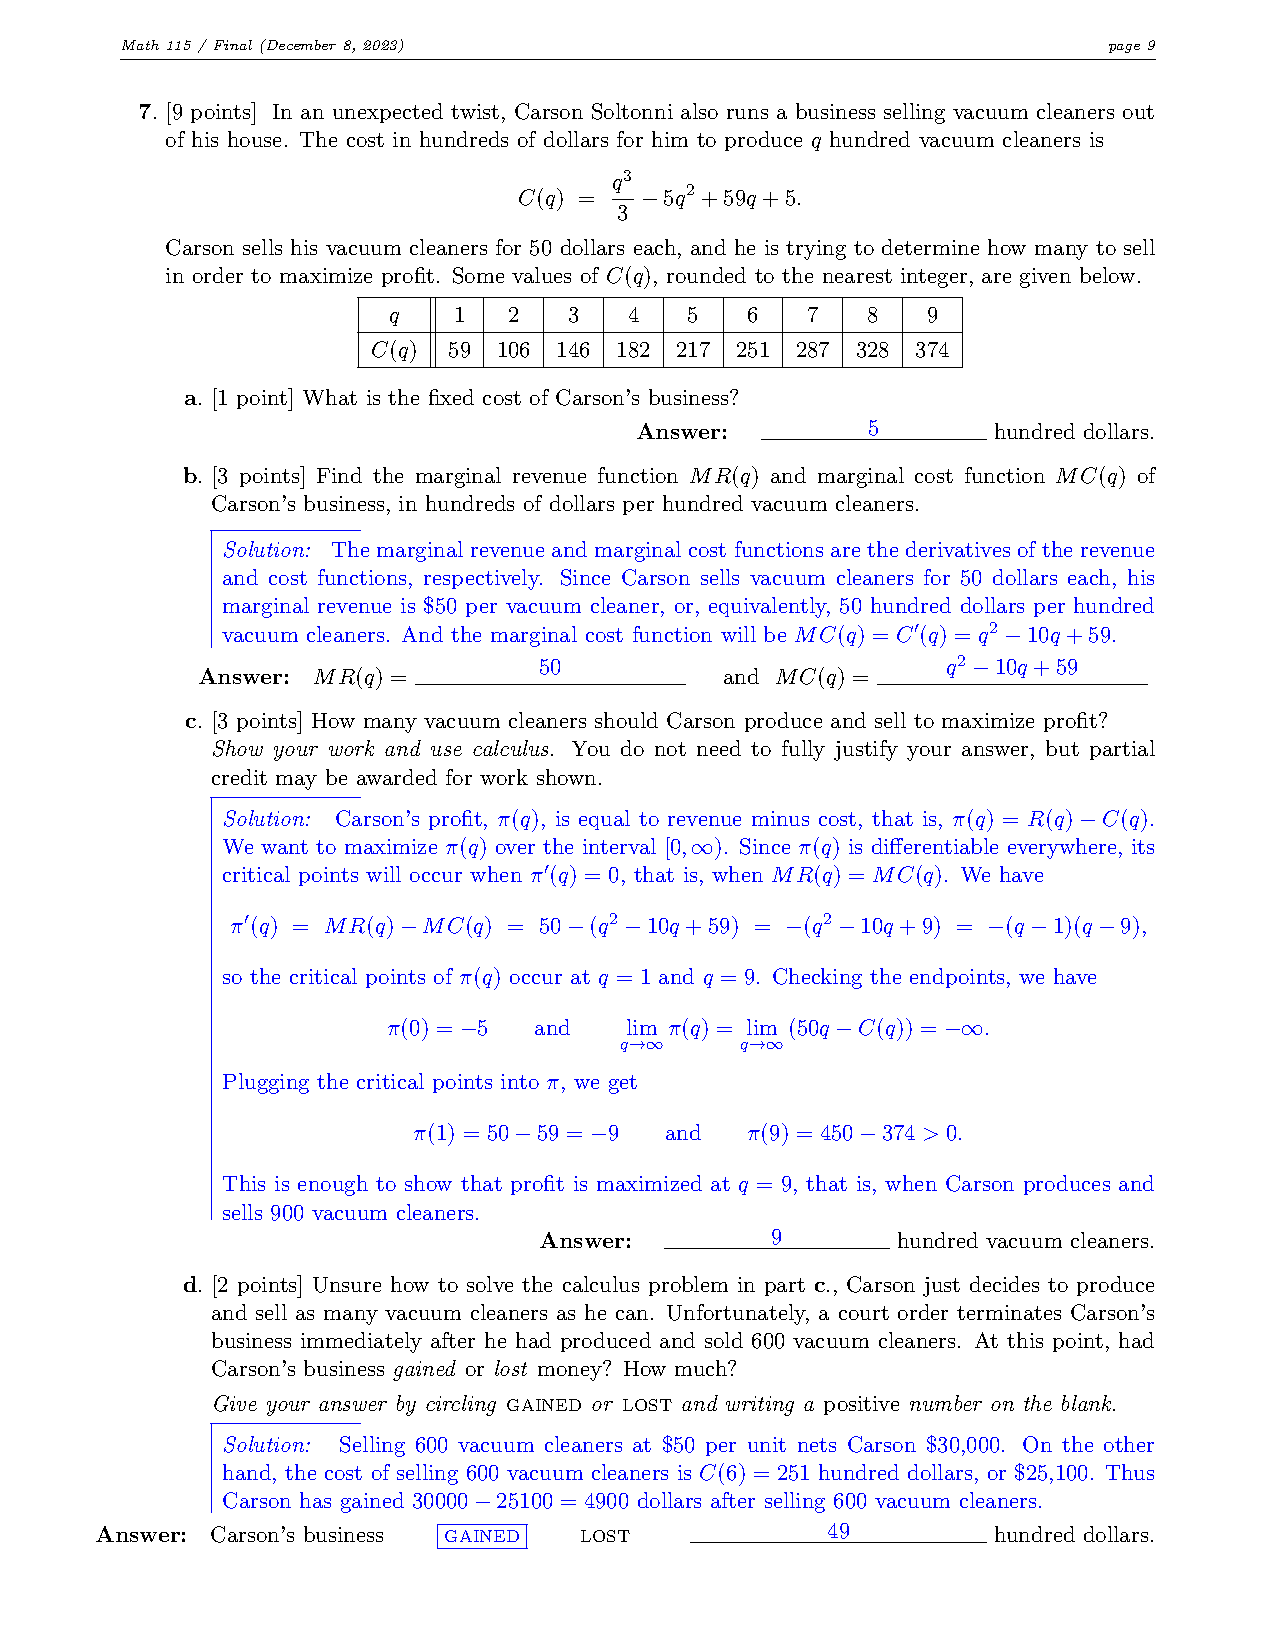
\includepdf[pages=-,pagecommand={}]{Figures/s7-2.pdf}
    \else
    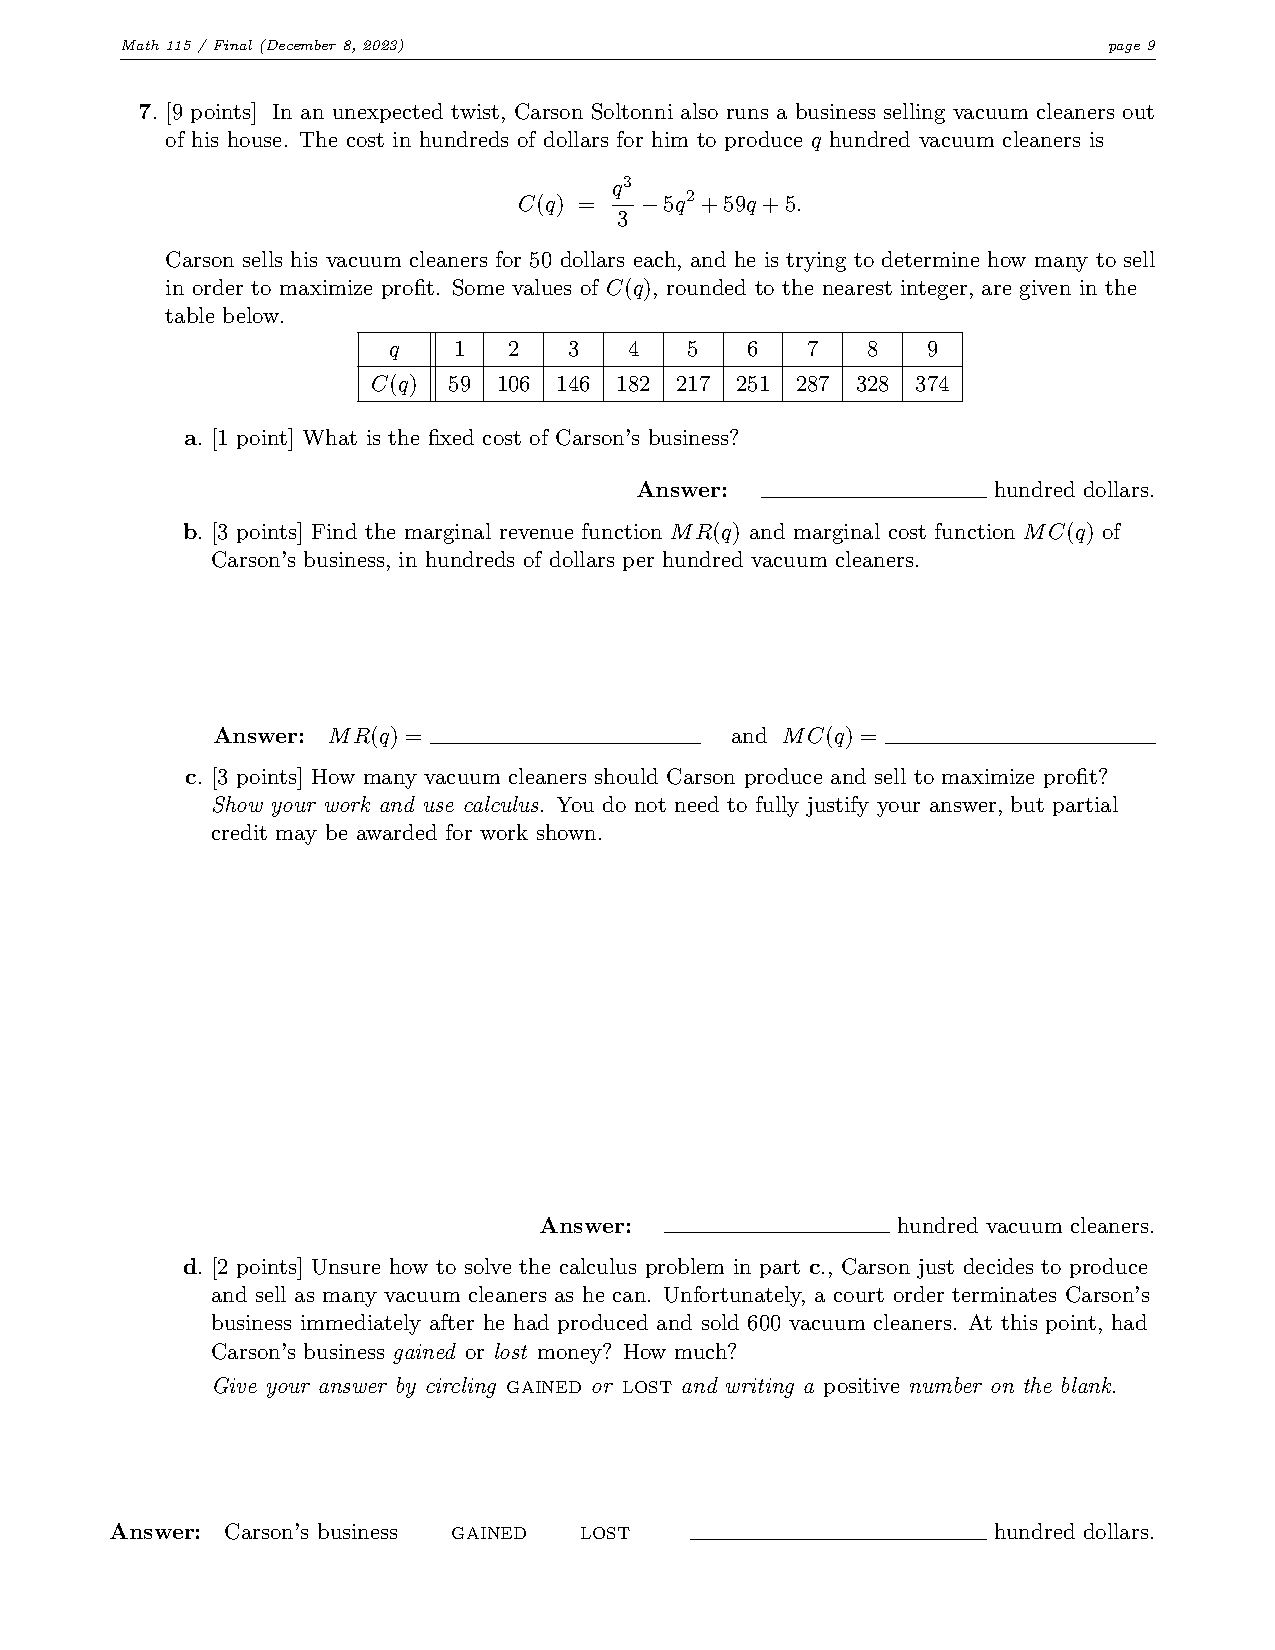
\includepdf[pages=-,pagecommand={}]{Figures/p7-2.pdf}
    \fi
\pagebreak
    \ifprintanswers 
    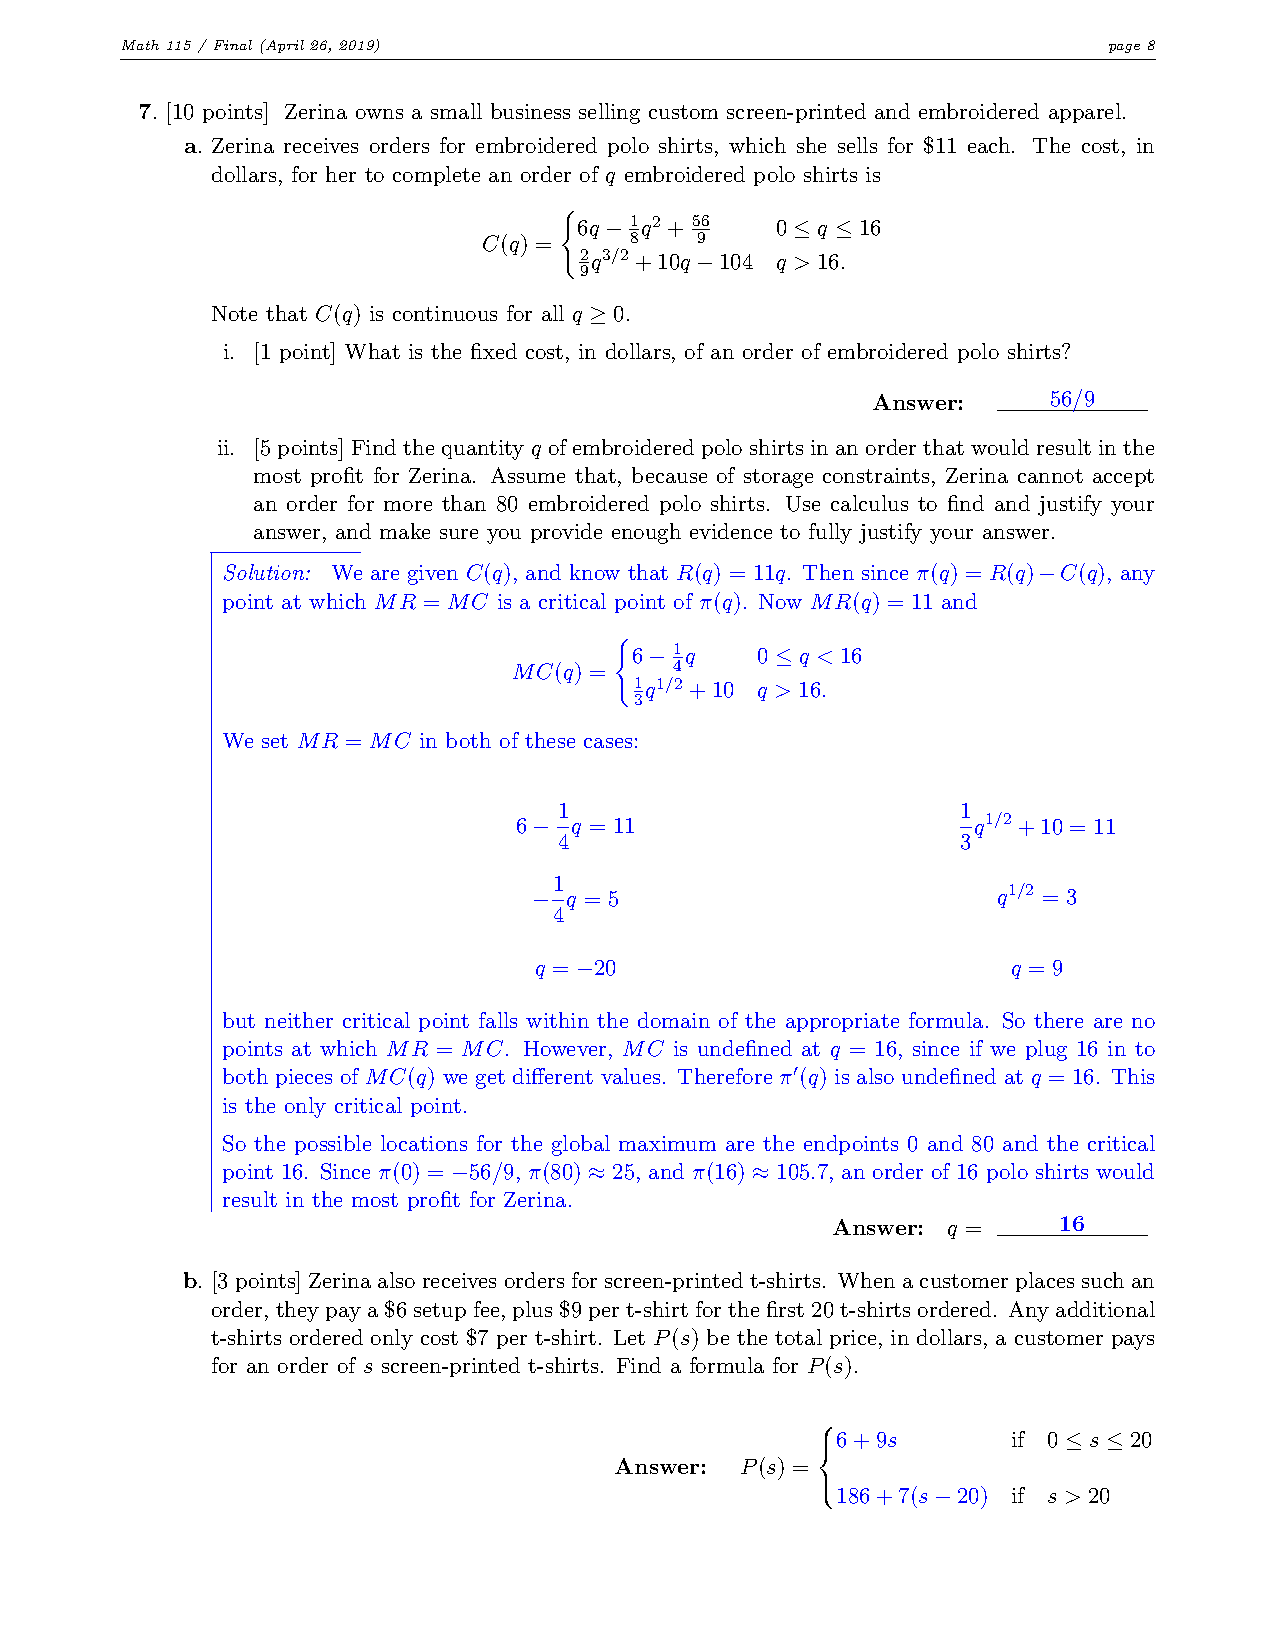
\includepdf[pages=-,pagecommand={}]{Figures/s7-3.pdf}
    \else
    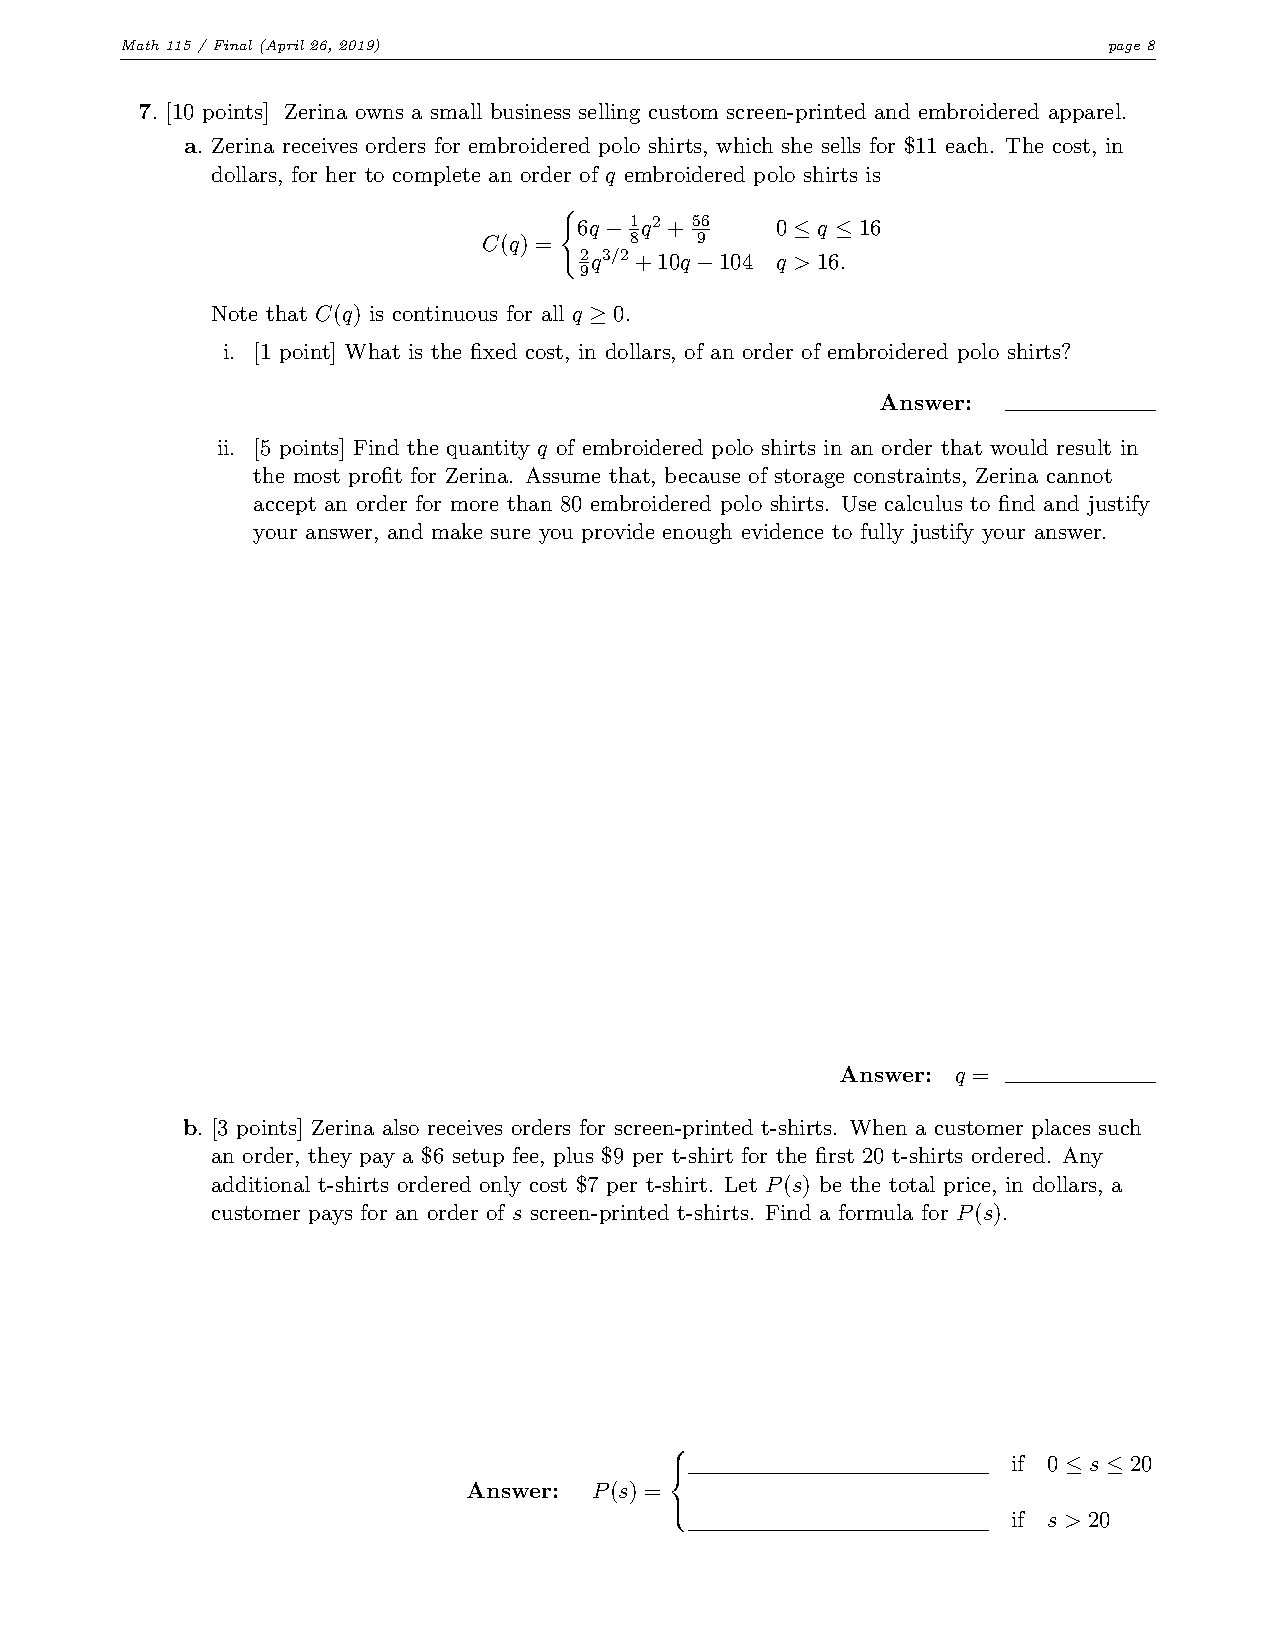
\includepdf[pages=-,pagecommand={}]{Figures/p7-3.pdf}
    \fi
\pagebreak
    \ifprintanswers 
    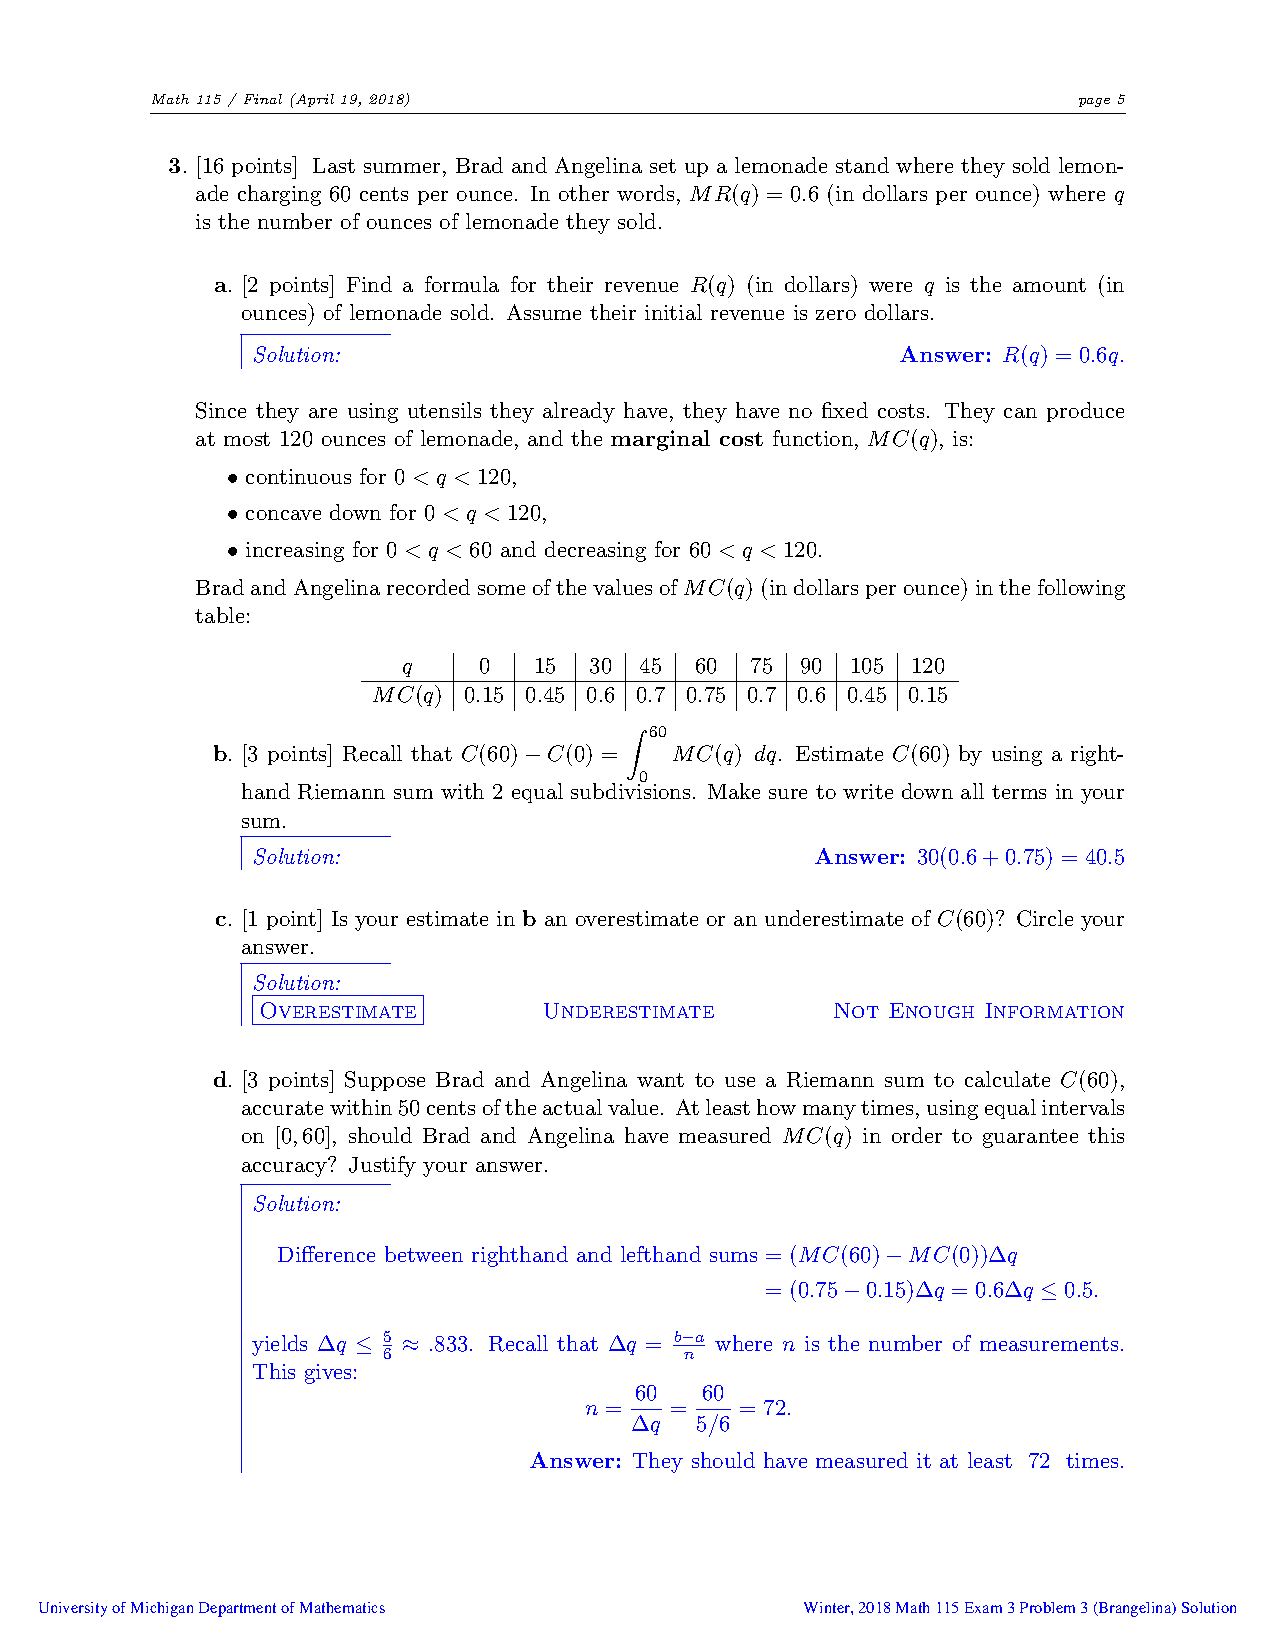
\includepdf[pages=-,pagecommand={}]{Figures/s3.pdf}
    \else
    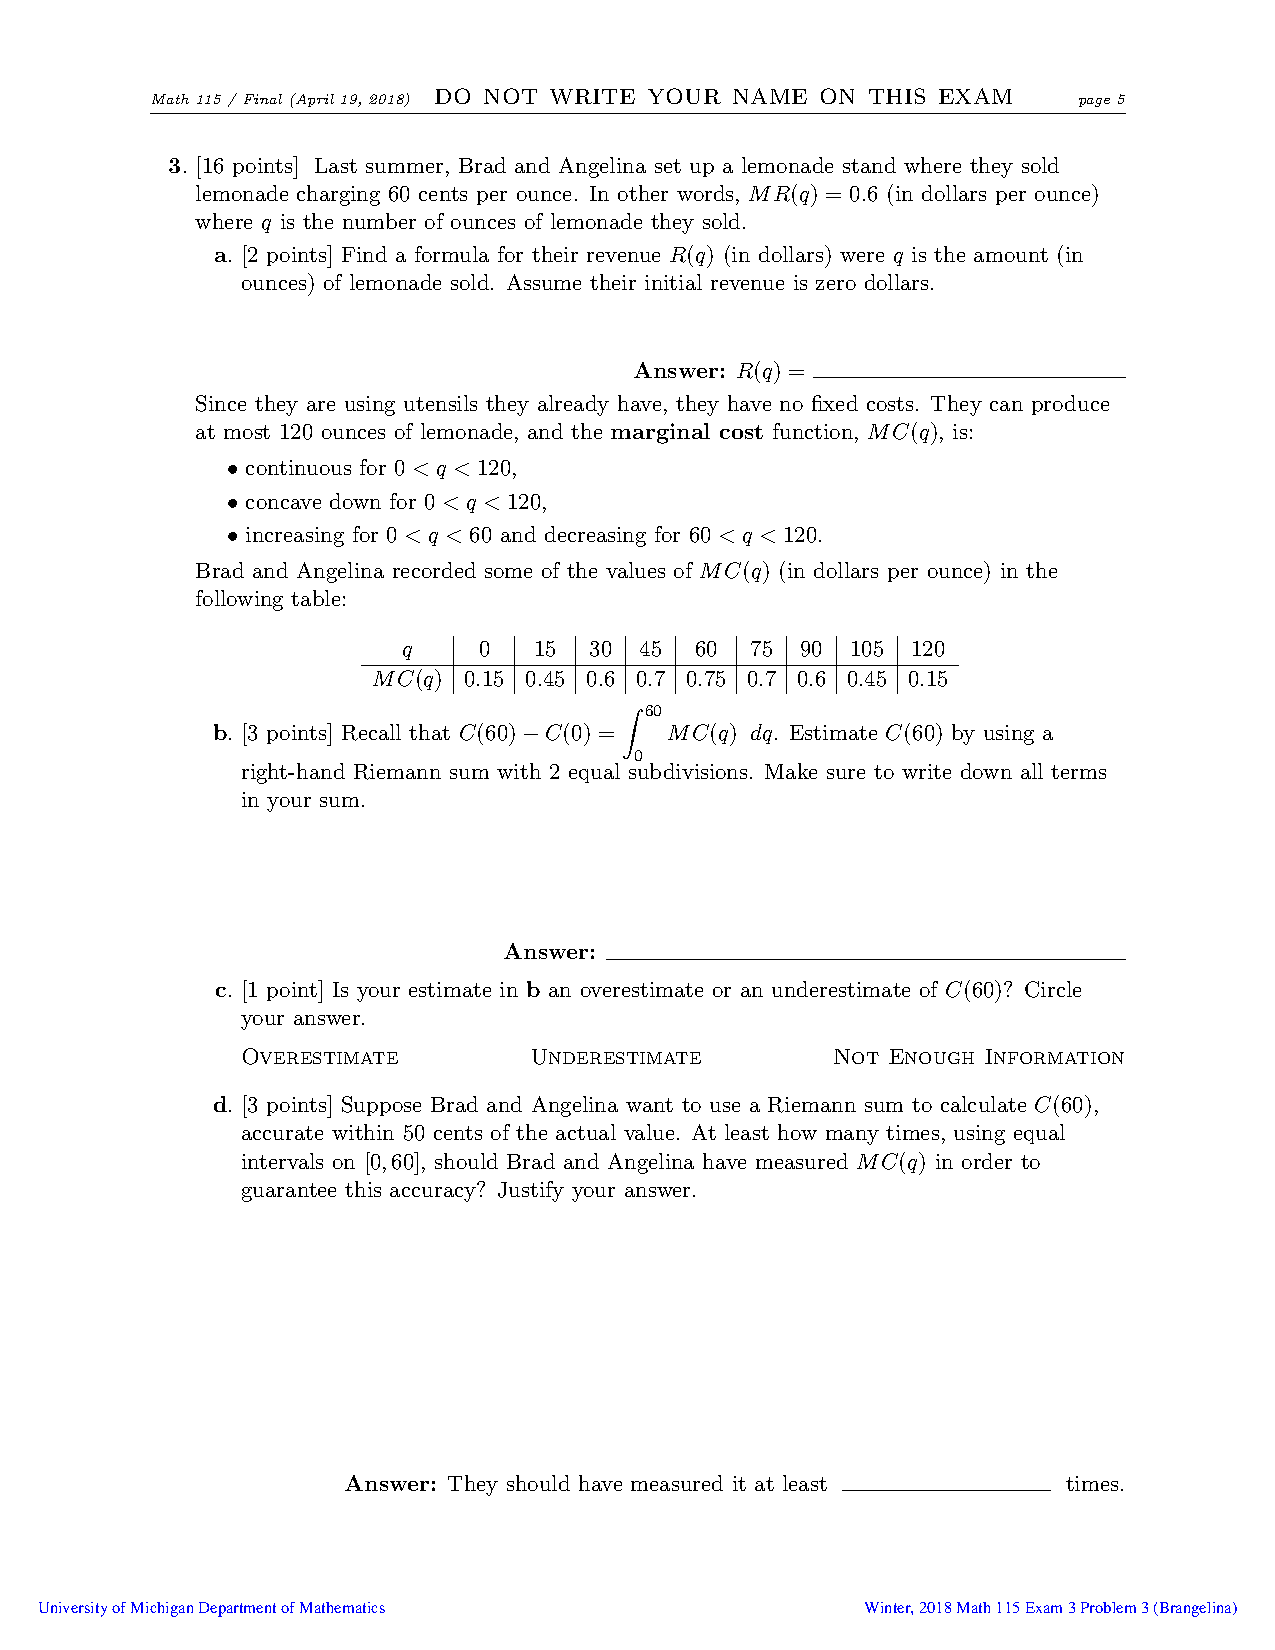
\includepdf[pages=-,pagecommand={}]{Figures/p3.pdf}
    \fi
\end{document}
%%% Local Variables:
%%% mode: latex
%%% TeX-master: t
%%% End:
